\chapter{Euclidea environment for solving geometric construction problems}
\label{euclidea_chapter}
In this chapter, we describe Euclidea, an online geometric construction game. The game is played with construction tools, which are used to complete various geometric problems. We will then present our version of Euclidea and describe how to apply random transformations to existing levels to create new variants of the same level.

\begin{figure}[h]
\centering
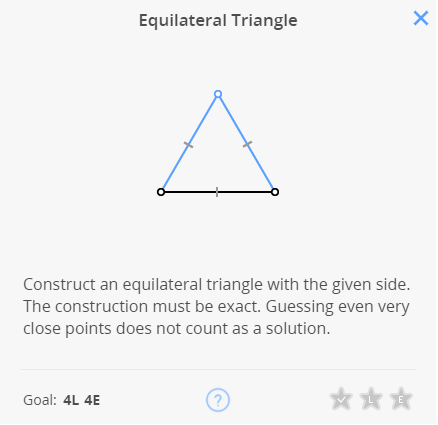
\includegraphics[width=70mm]{img/Actual_euclidea_definition.png}
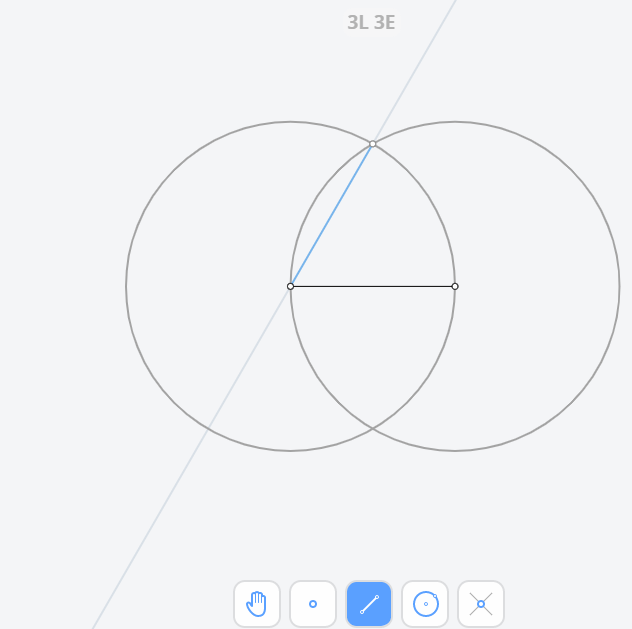
\includegraphics[width=70mm]{img/Actual_euclidea_screen.png}
\caption{Screenshot from Euclidea \cite{euclidea}. The goal of this level is to construct an equilateral triangle with the given side. The figure contains the goal description on the left and the construction on the right. The current state of the construction cost is 3L and 3E. Each usage of a tool costs pre-defined L cost and E cost. To get to the current state 3 tools were used: 2x Circle tool and 1x Line tool. Each tool costs 1L and 1E (see \ref{about_euclidea}).}
\end{figure}
\section{Euclidea}
\label{about_euclidea}
Euclidea is an online geometric construction game in 2-dimensional Euclidean space. In Euclidea we use the following terms:
\label{basic_concepts}
\begin{itemize}
    \item \textbf{Geometric primitives}  in Eculidea are points, lines and circles.
    \item \textbf{Level} in Euclidea is a geometric problem. Each level starts with an initial configuration, and the goal is to get to a target configuration.
    \item \textbf{Target configuration} denotes a state of a level that has all goals constructed, e.g.~it is done.
    \item \textbf{Goal description} is a definition of the remaining goals. In Euclidea, it is a visual information on how the remaining goal looks like. In our visualization marked as green lines, circles or points.
    \item \textbf{Current configuration} denotes a current state of construction, e.g~ it is initial configuration plus all constructed primitives with tools.
    \item \textbf{Initial configuration} denotes the first state of a level, and it also contains a goal description.
    \item \textbf{Scene}, \textbf{level instance} is generated by applying random transformations to the one predefined level template.
\end{itemize}
The main goal is to find a sequence of construction steps leading from an initial configuration of objects to a given target configuration. The construction steps utilize a set of straightedge and compass based tools (see Section \ref{euclidea_tools}). The game has two additional goals (L and E) and one hidden goal (V). The additional goals are to minimize L or E costs. The L cost is 1 for each tool used, with the exception of Point, Move, and Intersection tools, which have zero cost. The E cost equals the number of lines and circles necessary to construct the tool. The hidden goal is to find all possible solutions to a level and is thus available only for levels with multiple solutions.
\newline \newline
Every tool takes up to 3 arguments with values specified by coordinates of clicks on the image of the scene, for example, $circletool(A, B)$, where $A$, $B$ are points on the image of the scene. An exception is the Move tool, which is realized by dragging points to another place, although it can be represented also by a translation vector, defined by two click coordinates.
\newline \newline
Euclidea is divided into 15 level packs (Alpha, Beta, Gamma, \dots, Omicron) with increasing difficulty. Each level pack contains around 10 levels with a similar focus. Description of levels from Alpha to Zeta can be found in Appendix \ref{appendix_ch1} see Table \ref{level_descriptions}.
\section{Precision and goal evaluation}
\label{euclidea_precision}
In Euclidea, each level has its analytical model, which is projected on an image canvas. Each pixel in the image thus corresponds to a point in the analytical model. However, the analytical model points have float coordinates, making it impossible to find out precise coordinates of a point in the analytical model based on image data. Euclidea therefore provides certain tolerance for clicks and automatically finds the nearest geometric primitive corresponding to the click coordinates. 
\newline \newline
Euclidea checks the goal on the analytical level, so the player cannot cheat by drawing a similar goal instead. The player has to construct the target configuration to ensure that the result is the same as the goal.
\newline
\newline
In practice, the float parameters of two same geometric primitives stored in different objects cannot be the same, so even this comparison has some tolerance. We have to keep this float tolerance in mind because it might cause issues, as described in the chapter about data generation (see Section \ref{data_generation}).
\section{Tools}
\label{Euclidea_tools}
This section describes the tools available in Euclidea. They can be divided into 3 categories: Tools creating points, construction tools for lines and circles and the Move tool.
\label{euclidea_tools}
\subsection{Point and Intersection tools} \label{point_tool}
The Point tool takes one argument and creates a point in the desired location. However, in accordance with the precision approach in Euclidea (see Section \ref{euclidea_precision}), this tool also finds all line and circle primitives within a small neighborhood of the click coordinates and creates a point using the first applicable rule from the following:
\begin{enumerate}
  \item Create a point on the closest intersection of primitives if there are any.
  \item Create a point on the closest geometric primitive if there are any.
  \item Create a point at the exact coordinates given by the argument.
\end{enumerate}
\newline \newline
The Intersection tool creates points on all intersections of the two geometric primitives given in arguments. 
Both tools have E and L costs equal to 0.

\subsection{Construction tools}
The following tools take several arguments. Before a tool is executed, each click coordinates in the arguments are assigned the nearest geometric primitive matching the argument type.
\begin{table}[!htb]
\begin{center}
 \begin{tabular}{| m{2.7cm}| m{3.8cm} | m{5.2cm}| c{0.5cm} | c{0.5cm} |} 
 \hline
 \bfseries Tool &
 \bfseries Arguments &
 \bfseries Description & \bfseries L  &
 \bfseries E  \\
 \hline
 Line &
 (point, point) &
 Draw a line passing through the given points. &
 1 & 1 \\
 \hline
 Circle &
 (point, point) &
 Draw a circle centered at the first point with a radius marked by the second point.
 & 1 & 1 \\
 \hline
 Perpendicular Bisector &
 (point, point) &
 Draw the perpendicular bisector of two given points. & 1 & 3 \\
 \hline 
 Angle Bisector &
 (point, point, point) &
 Draw the axis of an angle, where the second point marks the vertex and the first and the third points lie on its rays. &
 1 & 4 \\
 \hline
 Perpendicular &
 (line, point) &
 Draw a line perpendicular to the line passing through the point. &
 1 & 3 \\
 \hline
 Parallel &
 (line, point) &
 Draw a line parallel to the line passing through the point. & 1 & 4 \\
 \hline
 Compass &
 (point, point, point) &
 Draw a circle with a center in the third point and a radius given by the distance between the first two points. &
 1 & 4 \\
 \hline
 %Intersection &
 %(line or circle, line or circle) &
 %Create points on all intersections of the two given geometric primitives. & 0 & 0\\
 %\hline
\end{tabular}
\caption{Tools available for construction steps in Euclidea. L and E denote the tool costs (see Section \ref{about_euclidea}).}
\end{center}

\end{table}

\subsection{Move tool}
\label{move_tool_definition}
The Move tool does not add any new geometric primitive but instead moves one primitive elsewhere and then recomputes the whole analytical model, if necessary. For example, if we move a line, the Move tool must also move all points on that line. Furthermore, it also has to adjust all the primitives intersecting those points, and so on. In Euclidea, the Move tool is used for exploring and understanding a given level. However, each level specifies the set of movable primitives, so not every primitive can be moved.
\newline
\newline
If a level configuration has multiple solutions, moving the primitives might remove some of the solutions. We will discuss this problem in data generation (see Section \ref{data_generation}).

\section{Our Euclidea-like environment}
In this thesis, we use our python version of Euclidea based on \cite{py_euclidea}, which contains every level and implements every tool.

\section{Example construction}
\label{euclidea_vizualization}
Each state in our environment is represented by two gray-scale images: the current configuration and the target configuration. The two images are stacked into an RGB image, where the red channel is the current state, and in the green are remaining goals, and the blue channel is filled with zeros. 

Figure \ref{EuclideaExample} shows an example of a level in our environment and the construction steps. The task of the level is to construct an equilateral triangle given by one side.

\begin{figure}[h!]
\begin{tabular}{ll}
\subfloat{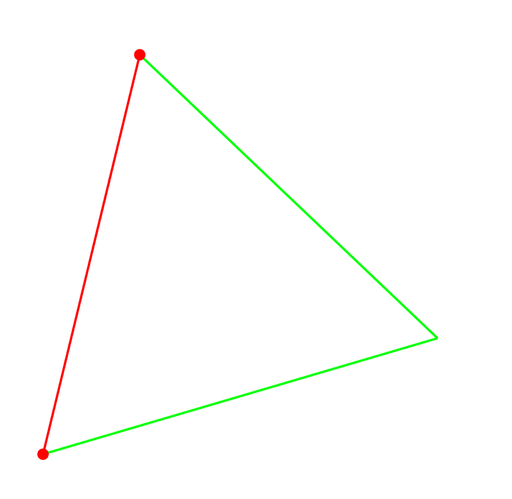
\includegraphics[width = 2.6 in]{img/Equilateral_example/input_image0.png}} &
\subfloat{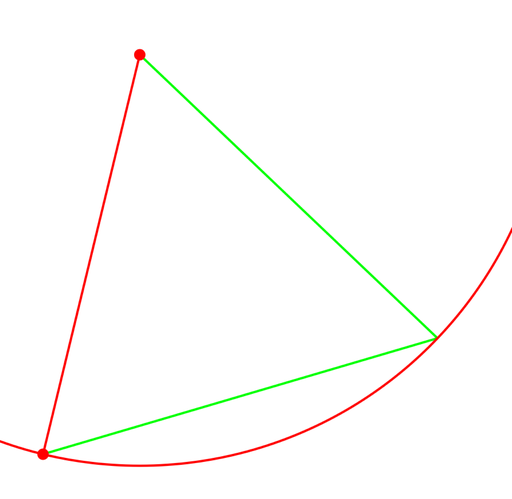
\includegraphics[width = 2.6 in]{img/Equilateral_example/input_image1.png}}\\

 a) Initial configuration & b) Construction step:1 \\

\subfloat{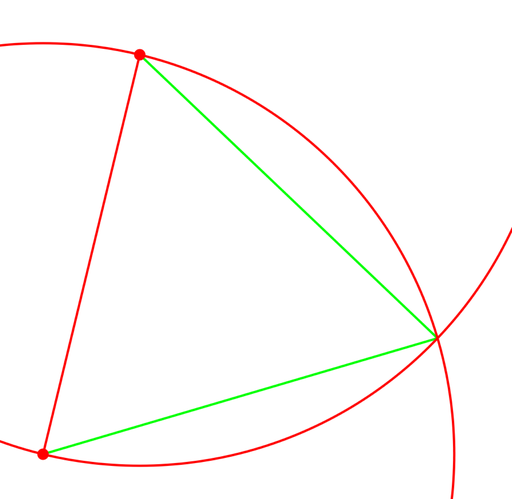
\includegraphics[width = 2.6 in]{img/Equilateral_example/input_image2.png}} &
\subfloat{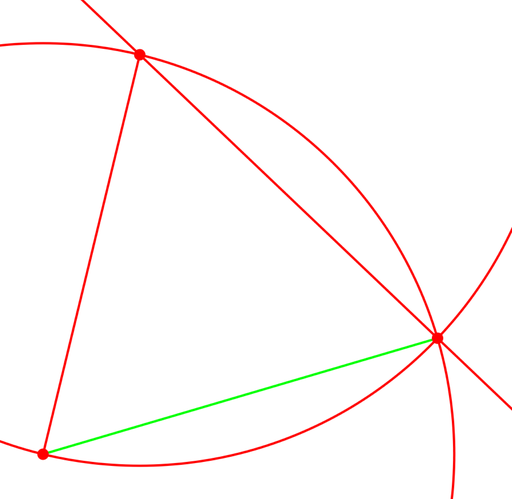
\includegraphics[width = 2.6 in]{img/Equilateral_example/input_image3.png}}\\

c) Construction step: 2 & d) Construction step:3 \\
\subfloat{
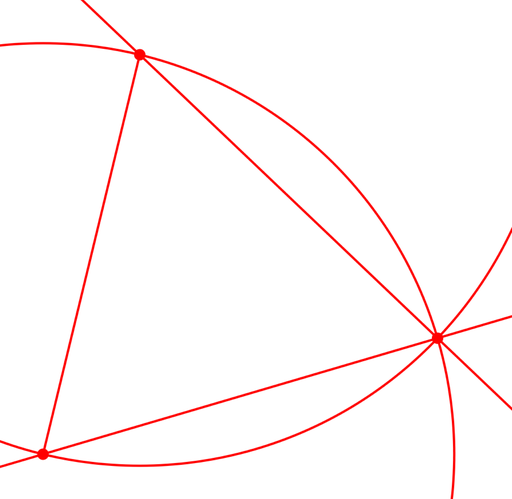
\includegraphics[width = 2.6 in]{img/Equilateral_example/input_image4.png}}
&
%\subfloat{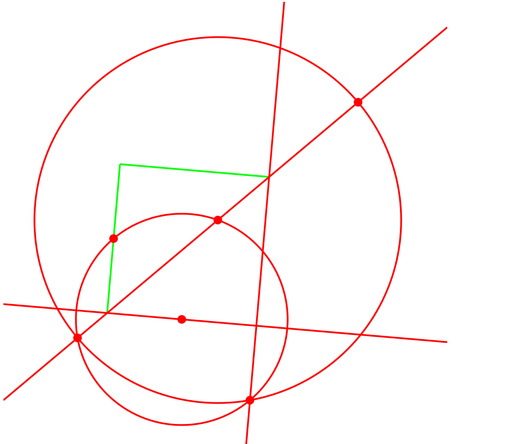
\includegraphics[width = 2.6 %in]{img/Equilateral_example/input_image5.png}}
\\

e) Construction step: 4 - level finished&  \\


\end{tabular}
\caption{Construction steps in our version of Euclidea for level \textit{Alpha-05}: Equilateral Triangle. Current state (red) and remaining goals (green). The first state is the level definition. In each step, we use one tool to construct the goal. Note that in Euclidea, we can see the goal, but we cannot use it for construction.}
\label{EuclideaExample}
\end{figure}

\section{Generation of level instances} \label{data_generation}
\label{data_gen_ref}
To train an automatic recognizer, we add a generator of new level instances to our version of Euclidea. The new scenes are based on predefined ones. Each level has one predefined scene and goal definition. In order to generate a new scene, we transform the predefined scene using the Move tool (see Section \ref{euclidea_tools}). Generated scenes can be either valid or degenerated. Degenerated scenes cannot be solved due to precision problems or other construction problems. We will describe how to recognize degenerated scenes in the rest of Section \ref{data_generation}.
\newline \newline
We use the following steps to generate training data:
\begin{enumerate}
  \item Load predefined scene.
  \item Apply random rotation.
  \item Randomly move all movable points.
  \item Apply random scale. 
  \item Check scene validity / degeneration.
  \item Apply random translation.
\end{enumerate}
There are two types of geometric primitives in the predefined scenes: constrained and movable. Constrained objects are constrained to another geometric primitive in the scene. We denote a construction of each constrained object as a ``step''. Objects constructed within one step can be constrained to any movable object or to an object constructed in previous steps.
An example of a constrained object is: ``point on a line'', ``line perpendicular to another line'' etc.
Movable objects on the other hand are not constrained to any other object, so they can be moved, but their movement also moves all other objects constrained to them. Our version of Euclidea contains only movable points. Circles and lines may be constrained to other points; note that these points can be hidden from the visualization of the level.
\newline \newline
The generation process can lead to degenerated scenes, i.e.~scenes that cannot be solved based on image information, mainly because certain parts are too close to each other and cannot be distinguished. Additionally, during re-scaling, we compute a minimal possible scale to avoid small scenes degenerated due to a small size.
 
\subsection{Degeneration criteria}
\label{degen_criteria}
Degeneration criteria are a set of rules that attempt to determine whether a scene is degenerated. 
We use the following four rules:
\begin{enumerate}
  \item Different points cannot be too close to each other, measured in pixels.
  \item Circles cannot have a too small radius, measured in pixels. 
  \item Two lines with a similar cannot be too close. Normal vectors compared in the analytical model.
  \item Intersections of geometric primitives can not be too close to points used in the construction, measured in pixels.
\end{enumerate}
The Rule 4. was added later as it is mainly used in the advanced Euclidea levels.
Rules number 1.-3.~were at first only applied to geometric primitives that were in the level definition. However, the degeneration status of a level definition does not include the degeneration of construction. So construction degeneration has to be checked as well. There is possibly an infinite number of different constructions, and we cannot make them all valid. 
\newline \newline
Without rule 4.~the degeneration criteria had two significant problems that led to degeneration:
\begin{itemize}
  \item Levels with multiple solutions can have configurations that make those solutions coalesce into each other. Probability of this generation goes to $0$, but those solutions can be so close together that we cannot differ one from another based on visual information.
  \item During construction, we create many intersections between geometric primitives. Although we force points created during construction to be reasonable by previous rules, we force only those points that are necessary for the construction. Sometimes a point not necessary for the construction can be too close to a construction point.
\end{itemize}
The second problem is more general than the first one, and the solution to it also solves the first problem. To realize rule 4.~we go through all intersections between all pairs of primitives and check if they are far enough from important points.
\newline \newline
As we found out, for some levels these degeneration rules do not ensure validity and we need to define level-specific degeneration criteria as described next.  

\subsection{Level-specific degeneration criteria}
Certain levels require degeneration rules that are not general. Some definitions of the levels also have ``additional degeneration'' which is again a set of rules applied only for instances of that level. The most frequent use of those additional degeneration rules is that specific angles cannot be too small or obtuse. It is also used to add additional constraints between objects of the scene that are level-specific. For example, in one level that contains two squares, those squares should not overlap.
\subsection{Precision problems}
While generating data, especially the constructions, we also have to deal with precision problems tied with scene re-scaling.  Generally, when we create a construction, we have to check whether two primitives are the same.  Each primitive is defined by a number of normalized arguments. An object with parameters $args_1$ is identical to an object with parameters $args_2$ when:
\begin{equation}
|args_1 - args_2| < \epsilon
\end{equation}
However, the difference can surpass $\epsilon$ when the objects are upscaled. Then objects are considered the same, but they are not. This can also occur the other way around. This may generate different construction then then desired. This precision problem has to be dealt with during the construction creation. However, it is only present when a level can have multiple solutions that can be potentially very close.
